\chapter{Roofline 性能模型}\label{v0ch:22}
\begin{chaptersummary}
算法已能求出解，下一步是解释运行时间由什么限制。本章以算术强度连接计算吞吐和数据搬运，建立 Roofline 的可检验上界。后续各离散方法都用同一口径分析，但工作量、缓存层级和测量范围必须一致。核心是先识别瓶颈，再选择能够改变该瓶颈的优化。
\end{chaptersummary}
\learninggoals{计算 FLOPs、字节与 ridge point；区分理论峰值、持续带宽和实测吞吐；解释 GEMM 与 SpMV 的差别。}
\paragraph{核心问题}同样执行浮点运算，为何不同核函数的吞吐相差很大？

\section{两个资源上界}
设工作量 $F$ FLOPs、选定内存层级的数据流量 $Q$ bytes、持续带宽 $B$ bytes/s、相应精度峰值 $P_{\rm peak}$ FLOP/s，则
\[
 I=F/Q,\quad P_{\rm attained}=F/T,\qquad
 P_{\rm attained}\le\min(P_{\rm peak},BI),\qquad
 I_{\rm ridge}=P_{\rm peak}/B.
\]
Roofline 以横轴算术强度、纵轴吞吐呈现资源上界。\cite{roofline}
模型是现代性能分析的组织工具；计算、存储与通信限制本身早于该模型。延迟、依赖、指令混合、并行度和负载不均会使实际点低于上界。
处理器通过流水线、向量单元、多核与加速器提高算术吞吐，而主存延迟与可用带宽未必按相同比例增长，形成所谓 memory wall。缓存、分块和批量计算通过复用缓和失衡；machine balance $P_{\rm peak}/B$ 则给出转入计算受限所需的强度尺度。\cite{architecture}
计算峰值利用率为 $P_{\rm attained}/P_{\rm peak}$；相对 Roofline 利用率为 $P_{\rm attained}/\min(P_{\rm peak},BI)$。两者必须使用相同精度、工作量与流量口径，不能混为一个效率数值。
\conceptbridge{为什么不能只统计执行了多少次加乘？}{相同算术可能反复使用寄存器中的数据，也可能每次都等待新数据。算术强度把工作量与所选层级的数据搬运联系起来。只减少 FLOPs 可能不减少关键流量，甚至降低吞吐指标却缩短时间。}{算子工作量 $\longrightarrow$ 数据复用 $\longrightarrow$ 受限资源与运行时间。}
\section{GEMM 与 CSR-SpMV}
稠密方阵乘 $C=AB$ 约 $2n^3$ FLOPs；理想每个输入读一次、输出写一次，双精度流量约 $24n^2$ bytes，故理想强度约 $n/12$。实际缓存容量、分块和写分配会改变流量。
CSR-SpMV 每非零元按一次乘加计 2 FLOPs。双精度值与 32 位列索引至少需 12 bytes，再加行指针、$\bm x$ 访问及输出；即使 $\bm x$ 大量复用，强度通常仍较低。具体字节模型由索引宽度、缓存命中和访问方式确定。
\section{估算、计时与标定}
本卷示意图设 $P_{\rm peak}=1000$ GFLOP/s、$B=100$ GB/s，ridge 为 10 FLOP/byte，用于展示屋顶的几何含义。CPU 核函数图则依据实际计时与工作量模型绘制；定位本机性能点时，应另行标定相应硬件屋顶。
\begin{figure}[htbp]\centering
\IfFileExists{Vol0_Linear_Algebra_HPC/figures/roofline_model.pdf}{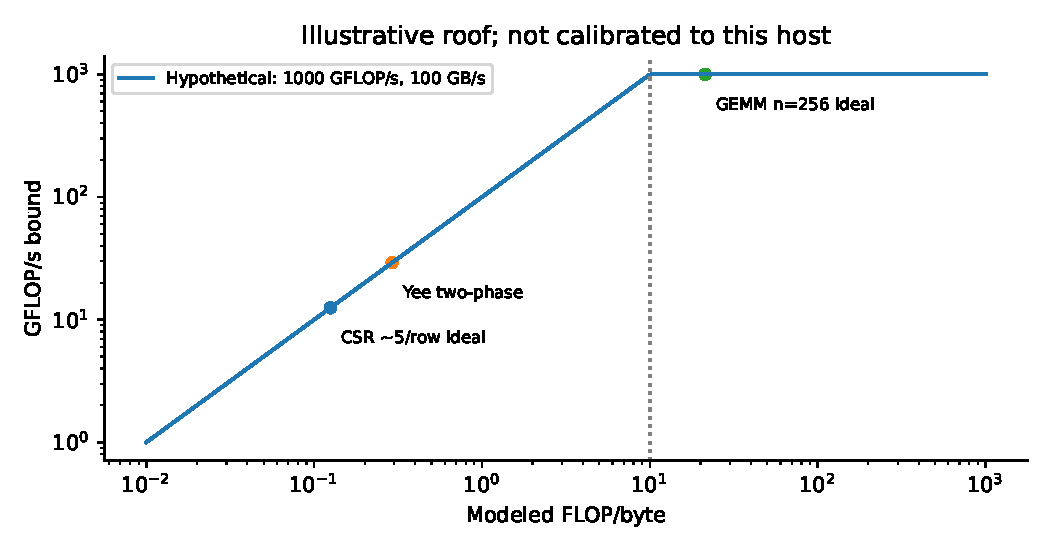
\includegraphics[width=.84\textwidth]{Vol0_Linear_Algebra_HPC/figures/roofline_model.pdf}}{}
\caption{假设硬件的 Roofline 示意；屋顶与字节模型均非 DRAM 计数器实测。}
\end{figure}
标定时需分别测持续带宽、对应精度计算吞吐及真实数据流量；不同缓存层级可建立不同屋顶。小数组驻留缓存时，DRAM 流量模型不适用。
\costnote{带宽受限核优先减少流量、改善复用与布局；计算受限核优先提升向量化和指令效率。GFLOP/s 用于定位资源利用，固定误差下的总时间用于评价计算收益。}
\coderef{roofline/kernels.py}
\aiexercise{对 32 位与 64 位索引 CSR 分别推导理想和逐非零读取 $x$ 的字节模型，计算强度，并说明写分配遗漏在哪里。}{给定 GEMM、SpMV 的实际计时和数组大小，判断能否把它们放到同一 DRAM Roofline；列出还缺的测量。}
\studyroute{略去硬件计数器校准与经验多层 Roofline 工具实现。参考 \cite{roofline,cuda}。}{arithmetic intensity; operational intensity; ridge point; sustained bandwidth; hierarchical Roofline}
